\documentclass[10pt]{report}
\usepackage{graphicx}
\usepackage{placeins}
\usepackage{colortbl}
\usepackage{algorithmic}
\usepackage{url}
\usepackage{algorithm}
\usepackage{listings}
\usepackage{flushend}
\usepackage{caption}
\usepackage{subcaption}
\usepackage{amssymb,amsmath}
\usepackage{tabularx}
\usepackage{array}
\usepackage{verbatim}
\usepackage{todonotes}
\usepackage{multirow}

\renewcommand*\thesection{\arabic{section}}

\begin{document} 
%
% paper title
% can use linebreaks \\ within to get better formatting as desired
\title{Guide: Elastic Cassandra Setup}
% author names and affiliations
% use a multiple column layout for up to three different
% affiliations
\author{
Daniel Moldovan\\
E-mail: d.moldovan@dsg.tuwien.ac.at}

\date{}

\maketitle

\tableofcontents
%\listoffigures 
 
 \newpage

\section{Introduction}


\begin{figure}
\centering
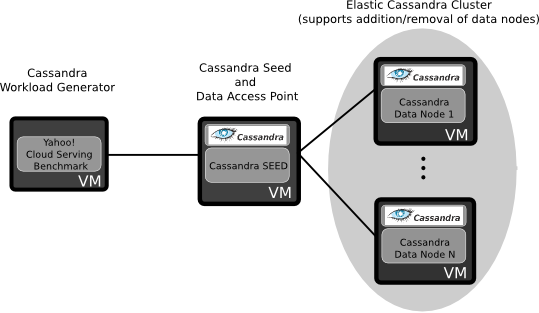
\includegraphics[width=\textwidth]{./topologyOverview.png}
\caption{Elastic Cassandra topology overview}
\label{fig:topologyOverview}
\end{figure} 

This guide explains how to setup Cassandra\footnote{\url{http://cassandra.apache.org/}} NoSQL distributed data store cluster using a set of scripts in order to behave elastically in a virtualized environment, by allowing dynamic addition and removal of Data Processing Nodes.

The general idea of our setup is to maintain a single Cassandra Node acting as Seed, representing the node to which any other Cassandra machines connect to and get a load token to join the Cassandra cluster, and support automated addition and removal of Data Nodes (\figurename~\ref{fig:topologyOverview}). Having this node alive throughout the lifetime of the Cassandra Cluster (from deployment up to when the cluster is decommissioned and all nodes destroyed), this node can also be considered as the data access point. While in this guide we assume there is only one Seed node, in practice one can setup using our scripts multiple Seed nodes, thus avoiding situations in which one data access machine can become a bottleneck. The supplied scripts can be used to configure Virtual Machine (VM) images as Cassandra Seeds, and other machines as Cassandra Data Nodes. When scaling out the system, the added Data Node machines automatically connect to the supplied Seed IP and join the Cassandra cluster, while when scaling in the cluster, we supply a mechanism for gracefully removing a Data Node from the cluster from the Seed machine.

One weak point could be that we use the default Cassandra token allocation mechanism, an advantage being that we obtain a shorter scaling out time, but possibly resulting in an unbalanced data distribution, since we do not rebalance the load across all data nodes. 

 To provide realistic workload for the data end, we provide scripts to be used in configuring a separate machine as Cassandra workload generator, running the Yahoo! Cloud Serving Benchmark (YCSB)\footnote{\url{http://research.yahoo.com/Web_Information_Management/YCSB}}, benchmark built to measure the performance (such as latency or throughput) of distributed data engines.


\section{Setup Elastic Cassandra}


\begin{figure}
\centering
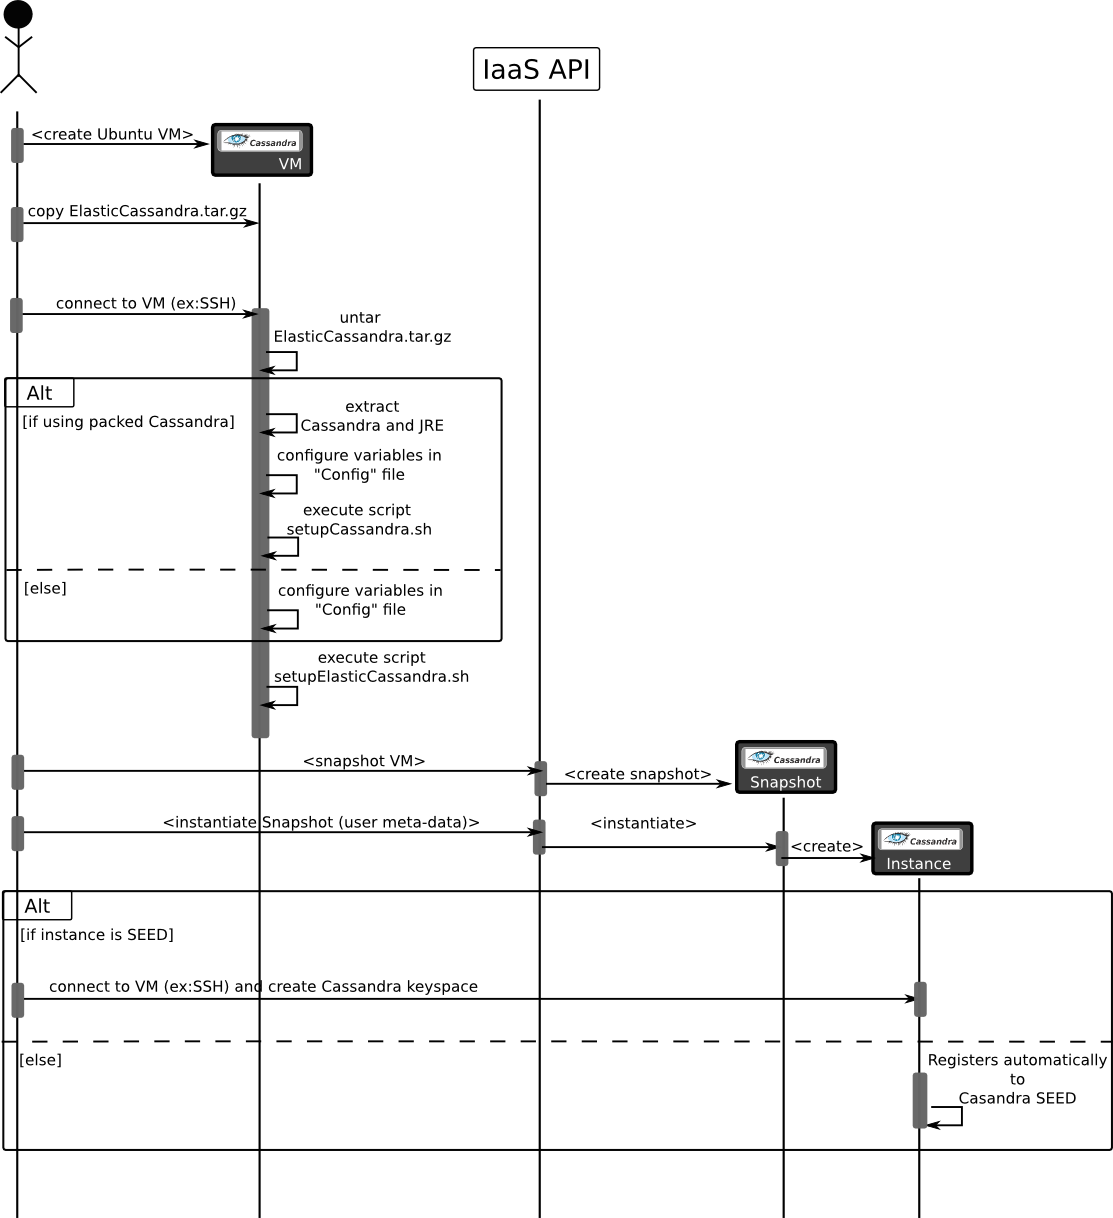
\includegraphics[width=\textwidth]{./sequenceDiagram.png}
\caption{Operations sequence for configuring Elastic Cassandra}
\label{fig:elasticitySignatureAnalysisReport}
\end{figure} 

We provide a series of scripts which configure a Cassandra setup to be elastic, supporting addition and removal of data processing nodes. The sequence of necessary operations for configuring Cassandra to be elastic is depicted in \figurename~\ref{fig:elasticitySignatureAnalysisReport}:

\begin{enumerate}
  \item A new virtual machine is created having Ubuntu as operating system. Actually, any Ubuntu-like system should work, as long as it maintains the same service definition mechanisms (init.d).
  \item One of the archives we provide is copied and extracted in the new virtual machine. We provide archives containing only our scripts, containing a pre-packed Cassandra, and containing a pre-packed Cassandra and JREs (x64 and X86).
  \item The user must untar the Cassandra and JRE archives, and change directory to "./ElasticCassandraScripts".
  \item The environment variables contained in the Config file must me configured. The variables are as follows:
    \begin{itemize}
    \item HOME: The directory in which the scripts are located.
    \item CASSANDRA\_HOME: Cassandra home directory.
    \item CASSANDRA\_BIN : Location of the Cassandra "bin" directory or binary files (cassandra, nodetool, etc).
    \item CASSANDRA\_CONFIG: Location of the Cassandra configuration files. 
    \item JAVA\_HOME: Root directory containing a standalone Java deployment.
     \item CASSANDRA\_SEED\_IP\_SOURCE: A script/bash command that can retrieve the SEED IP at system boot time (for example using contextualization mechanisms) or directly a comma separated values list. This source is used to configure Cassandra Nodes in order to connect directly to the SEED IPs when booting for joining the Cassandra cluster.    
    \end{itemize}  
 \item If the pre-packed Cassandra is used, the user must run the "setupCassandra.sh" script, which uses the supplied JAVA\_HOME to deploy a standalone Cassandra.
 \item The second "setupElasticCassandra.sh" script configures depending on the node type (Seed or Node) the Cassandra installation, as to enable addition and removal of data nodes at run-time. The script prompts the user to select if he wants to configure the respective machine as "Seed (Main Node)" or "Data Node (Slave)".
 \item The resulting Cassandra Seed or Data Node VM must be snapshotted BEFORE the Cassandra service is started, as to avoid the creation of load tokens. If a token is created, then no-mater how many VM's are instantiated using a snapshot, they will all have exact the same database load allocated to them, rendering the scale out process useless.
 \item If the configured machines do not need to be snapshotted, please reboot their OS (sudo reboot) as to start Cassandra properly, as our scripts are embedded in /etc/init.d and /etc/rc/.local and are configured to be executed during a normal boot sequence.
 \item For connecting to Cassandra using "cassandra-cli" , the host argument "-h" must point to the machine IP, not "localhost" (CASSANDRA\_PATH/bin/cassandra-cli -h IP)
 \item After creating a snapshot to serve as base for Cassandra Seed, the user can configure another machine as Data Node, by selecting, when prompted, the second option "setupElasticCassandra.sh" script option ("Data Node (Slave)"), having the CASSANDRA\_SEED\_IP\_SOURCE defined as a script which can retrieve data from a VM contextualization mechanism or as a static IP.  
 \item To start Cassandra properly on the Seed configured nodes, just reboot the OS. Mainly, /etc/rc.local is executed also at boot time, and calls a script which creates a Cassandra keyspace to be used by YCSB, and also configures some other Cassandra parameters.
 \item To test if the Cassandra cluster is working, from any Cassandra VM (preferably but not mandatory Cassandra Seed), execute :
 
  $CASSANDRA\_PATH/bin/nodetool~-h~localhost~ring$
  
  ,  which shows the IPs associated to a cluster, and their load distribution. Or use the supplied "checkCassandraStatus.sh" script, which execute the call described above. The output should show all your IPs associated to your cluster, but it might take some while (usually 30 seconds) after a Node boots until it starts joining the cluster. 
 \end{enumerate} 

\paragraph{Note}
 If Cassandra operations should be run on a machine configured as Cassandra Seed as to create a needed keyspace, the needed operations can be inserted in the "createCassandraKeyspaceScript.txt", which is run when Cassandra Seed machine boots, thus running any user-defined Cassandra operations. 

\section{Scale In/Out Elastic Cassandra Cluster}

After having a Cassandra cluster deployed, there are some simple steps to scale in and out the cluster.
\paragraph{Scaling In} For scaling in the cluster (\figurename~\ref{fig:scaleIn}), one must call in the Cassandra Seed machine (ex trough SSH) "decommission IP" (ex: "ssh HOST\_IP decommission TARGET\_IP"), which removes gracefully the node having the IP TARGET\_IP. This step is important as Cassandra needs to move data to ensure consistency and redundancy. After the "decommission" command terminates, the virtual machine having the TARGET\_IP can be destroyed using the used IaaS API.

\begin{figure}
\centering
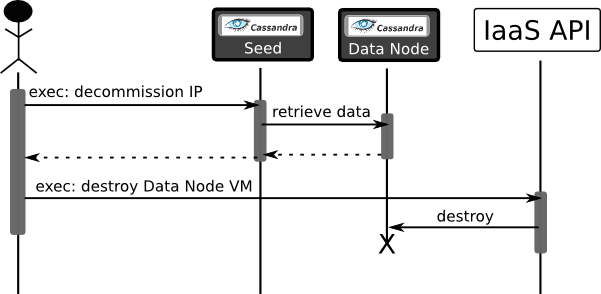
\includegraphics[width=0.8\textwidth]{./scaleIn.png}
\caption{Operations sequence for Scaling In Elastic Cassandra Cluster}
\label{fig:scaleIn}
\end{figure} 
 
 
\paragraph{Scaling Out} For scaling out the cluster (\figurename~\ref{fig:scaleOut}), our scripts configure the Cassandra Node to automatically connect to a supplied Seed IP, in order to obtain a load allocation token. In order to be able to connect to a Seed IP, the CASSANDRA\_SEED\_IP\_SOURCE entry in the "Config" file must be properly configured.


\begin{figure}
\centering
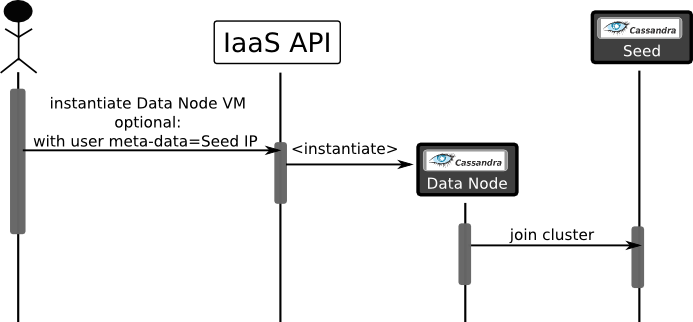
\includegraphics[width=0.8\textwidth]{./scaleOut.png}
\caption{Operations sequence for Scaling Out Elastic Cassandra Cluster}
\label{fig:scaleOut}
\end{figure} 

\FloatBarrier
%\section{Setup Yahoo! Cloud Serving Benchmark (YCSB)}

%The Yahoo! Cloud Serving Benchmark can act as a load generator for the Elastic Cassandra Cluster. We provide an archive containing an YCSB distribution. For configuring the YCSB machine, the user must:   
%\begin{enumerate}
%  \item Copy the YCSB archive and untar on a target virtual machine. We provide several archives, one containing only the YCSB and our scripts, and two including JDK-s for compiling YCSB (x64 and i586).
%  \item Change the current directory to "./ycsb". 
%   \item Set the environment variables contained in the Config file:
%    \begin{itemize}
%      \item JAVA\_HOME: Root directory containing a standalone Java JDK deployment
%      \item TARGET\_CASSANDRA\_IPs: A script/bash command that can retrieve  at system boot time the IPs that YCSB will stress (for example using contextualization mechanisms) or directly a comma separated values list.
%    \end{itemize}  
%    \item Run the "installYCSB.sh" script, which creates in init.d an YCSB service that can be started manually, and that also starts automatically at system boot. The script also compiles the YCSB using Maven\footnote{\url{http://maven.apache.org/}}, which needs to be installed on the machine running YCSB. We also modified the Maven Pom.xml to build only connectors to Cassandra, as YCSB supports multiple database systems.
%    \item After running the script, the YCSB service can be started (sudo service ycsb start), or the configured machine snapshotted and instantiated) in the case in which the target IPs are specified using some contextualization mechanism", and the YCSB will start at boot time.
  
%YCSB supplies several workloads in the "YCSB-main" "workload" folder, which, depending on the system under test, must be configured to generate more or less operations. The workloads are run in a continuous loop respecting the sequence presented in \url{https://github.com/brianfrankcooper/YCSB/wiki/Core-Workloads}, and is as follows:  A, B, C, F, D (Files workloada, workloadb, workloadc, workloadf, workloadd). Please configure the workloads appropriately by changing their properties, as to generate more or less operations, as needed.   

%The scripts supplied for configuring the Cassandra cluster also create the keyspace needed by YCSB in the machines configures as Seed, when /etc/rc.local is executed at machine boot under the "sudo" user, thus the configured Seed machines need to be rebooted or their snapshots instantiated and the database is created automatically.
  
% \end{enumerate} 
 
%TODO:
%so you need to make clear that "Cloud services" mean: cloud applications as well as cloud infrastructure/platform services offered by the provider.
%"Elasticity" should be explained clearly that "multi-dimensional elasticity"

\paragraph{Note}
%More distributions of our scripts including Cassandra and Oracle JVMs available at \url{http://www.infosys.tuwien.ac.at/prototypes/ElasticCassandra/}
 
% that's all folks
\end{document}
